\documentclass[10pt,a4paper]{article}
\usepackage[utf8]{inputenc}
\usepackage{amsmath}
\usepackage{amsfonts}
\usepackage{amssymb}
\usepackage{amsthm}
\usepackage{float}
\usepackage{mathtools}
\usepackage{geometry}[margin=1in]
\usepackage{xspace}
\usepackage{tikz}
\usepackage{mathrsfs}
\usetikzlibrary{shapes, arrows, decorations.pathmorphing, ducks, automata}
\usepackage[parfill]{parskip}
\usepackage{subcaption}
\usepackage{stmaryrd}
\usepackage{marvosym}
\usepackage{dsfont}
\usepackage{pgfplots}
\usepackage{enumitem}
\usepackage{calc}
\usepackage{tikz-cd}
\usepackage{hyperref}

\hypersetup{
    colorlinks,
    citecolor=black,
    filecolor=black,
    linkcolor=black,
    urlcolor=black
}

\newcommand{\st}{\text{ s.t. }}
\newcommand{\contr}{\lightning}
\newcommand{\im}{\mathfrak{i}}
\newcommand{\R}{\mathbb{R}}
\newcommand{\Q}{\mathbb{Q}}
\newcommand{\C}{\mathbb{C}}
\newcommand{\F}{\mathbb{F}}
\newcommand{\K}{\mathbb{K}}
\newcommand{\N}{\mathbb{N}}
\newcommand{\Z}{\mathbb{Z}}
\renewcommand{\P}{\mathbb{P}}
\renewcommand{\H}{\mathds{H}}
\renewcommand{\O}{\mathcal{O}}
\newcommand{\A}{\mathbb{A}}
\newcommand{\D}{\mathbb{D}}
\newcommand{\nequiv}{\not\equiv}
\newcommand{\powset}{\mathcal{P}}
\renewcommand{\th}[1][th]{\textsuperscript{#1}\xspace}
\newcommand{\from}{\leftarrow}
\newcommand{\legendre}[2]{\left(\frac{#1}{#2}\right)}
\newcommand{\ow}{\text{otherwise}}
\newcommand{\imp}[2]{\underline{\textit{#1.}$\implies$\textit{#2.}}}
\let\oldexists\exists
\let\oldforall\forall
\renewcommand{\exists}{\oldexists\;}
\renewcommand{\forall}{\;\oldforall}
\renewcommand{\hat}{\widehat}
\renewcommand{\tilde}{\widetilde}
\newcommand{\one}{\mathds{1}}
\newcommand{\under}{\backslash}
\newcommand{\injection}{\hookrightarrow}
\newcommand{\surjection}{\twoheadrightarrow}
\newcommand{\jacobi}{\legendre}
\newcommand{\floor}[1]{\lfloor #1 \rfloor}
\newcommand{\ceil}[1]{\lceil #1 \rceil}
\newcommand{\cbrt}[1]{\sqrt[3]{#1}}
\renewcommand{\angle}[1]{\langle #1 \rangle}
\newcommand{\dbangle}[1]{\angle{\angle{#1}}}
\newcommand{\wrt}{\text{ w.r.t. }}

\newcommand*\circled[1]{\tikz[baseline=(char.base)]{
      \node[shape=circle,draw,inner sep=2pt] (char) {#1};}
}

\DeclareMathOperator{\ex}{ex}
\DeclareMathOperator{\id}{id}
\DeclareMathOperator{\upper}{Upper}
\DeclareMathOperator{\dom}{dom}
\DeclareMathOperator{\disc}{disc}
\DeclareMathOperator{\charr}{char}
\DeclareMathOperator{\Image}{im}
\DeclareMathOperator{\ord}{ord}
\DeclareMathOperator{\lcm}{lcm}
\DeclareMathOperator{\aut}{Aut}
\DeclareMathOperator{\diag}{diag}
\DeclareMathOperator{\stab}{stab}
\DeclareMathOperator{\trace}{trace}
\DeclareMathOperator{\ecl}{ecl}
\DeclareMathOperator{\Span}{Span}
\DeclareMathOperator{\Gal}{Gal}
\DeclareMathOperator{\Aut}{Aut}
\DeclareMathOperator{\Frob}{Frob}
\let\div\relax
\DeclareMathOperator{\div}{div}
\DeclareMathOperator{\Div}{Div}
\let\Re\relax
\let\Im\relax
\DeclareMathOperator{\Re}{\mathfrak{Re}}
\DeclareMathOperator{\Im}{\mathfrak{Im}}
\DeclareMathOperator{\Frac}{Frac}
\DeclareMathOperator{\Pic}{Pic}

\let\emph\relax
\DeclareTextFontCommand{\emph}{\bfseries\em}

\newtheorem{theorem}{Theorem}[section]
\newtheorem{lemma}[theorem]{Lemma}
\newtheorem{corollary}[theorem]{Corollary}
\newtheorem{proposition}[theorem]{Proposition}
\newtheorem{conjecture}[theorem]{Conjecture}
\newtheorem{definition}[theorem]{Definition}

\definecolor{burgundy}{rgb}{0.5, 0.0, 0.13}

\tikzset{sketch/.style={decorate,
 decoration={random steps, amplitude=1pt, segment length=5pt},
 line join=round, draw=black!80, very thick, fill=#1
}}

\pgfplotsset
  {
    compat                   = newest,
    every tick/.append style = thin,
    width= 0.95 \textwidth,
  }

\title{Complex Dynamics}
\begin{document}
\section{Introduction}
\subsection{Classical Motivation: Newton's Method}
Newton's method (also called Newton-Raphson) is an algorithm for finding roots of a polynomial. If $p(z)$ is a polynomial, then we construct the auxiliary function $f(z) = z - \frac{p(z)}{p'(z)}$. We then pick some value $z_0$ and we iterate, so that $z_{i+1} = f(z_i)$. Sometimes, depending on $p$ and $z_0$, this sequence converges to some $z$, so that $z = z-\frac{p(z)}{p'(z)}$, i.e. $p(z) = 0$. We can view this graphically for real values of $z$ as follows:

\begin{figure}[H]
  \centering
    \begin{tikzpicture}
      \begin{axis}[xmin = -3, xmax = 7, ymin = -2, ymax = 4, restrict y to domain=-10:10, axis lines=middle, xtick={-3,-2,...,7}, ytick={-1,0,...,4}, axis equal]
        \node[burgundy, circle, draw, fill, scale=0.1, label={[burgundy]below:$z_0$}] (a) at (4, 2.6875) {};
        \node[scale=0.01] (b) at (2.6875, 2.6875) {};
        \node[burgundy, circle, draw, fill, scale=0.1, label={[burgundy]below:$z_1$}] (c) at (2.6875, 1.8378) {};
        \node[scale=0.01] (d) at (1.8378, 1.8378) {};
        \node[scale=0.01] (e) at (1.8378, 1.3239) {};
        \node[scale=0.01] (f) at (1.3239, 1.3239) {};
        \node[scale=0.01] (g) at (1.3239, 1.0727) {};
        \node[scale=0.01] (h) at (1.0727, 1.0727) {};
        \node[scale=0.01] (i) at (1.0727, 1.0048) {};
        \node[scale=0.01] (j) at (1.0048, 1.0048) {};

        \draw[burgundy, ->] (a) -- (b);
        \draw[burgundy, ->] (b) -- (c);
        \draw[burgundy, ->] (c) -- (d);
        \draw[burgundy, ->] (d) -- (e);
        \draw[burgundy, ->] (e) -- (f);
        \draw[burgundy] (f) -- (g);
        \draw[burgundy] (g) -- (h);
        \draw[burgundy] (h) -- (i);
        \draw[burgundy] (i) -- (j);

        \addplot+[samples=100, mark=none, domain=-3:-0.24, blue] {(2*x^3+1)/(3*x^2)};
        \addplot+[samples=100, mark=none, domain=0.25:5, blue] {(2*x^3+1)/(3*x^2)} node[right, pos=1] {$f(x) = \frac{2x^3+1}{3x^2}$};
        \addplot+[red, mark=none] {x};
      \end{axis}
    \end{tikzpicture}
  \caption{Newton's method for $p(z) = z^3-1$}
\end{figure}

It's not too hard to see that, no matter our starting choice of $z_0$, this process will always eventually converge towards $z=1$, and that $p(1) = 0$.

If instead we consider this iteration for \emph{complex} values of $z_0$, we might converge to different roots of $p(z)$, since $p$ also has two complex roots. It turns out that the question of deciding which root we will converge to is not easy, and in fact we can see which root will be converged to in the following convergence diagram\footnote{Courtesy of usefuljs.net/fractals/docs/newtonian\_fractals.html}
\begin{figure}[H]
  \centering
  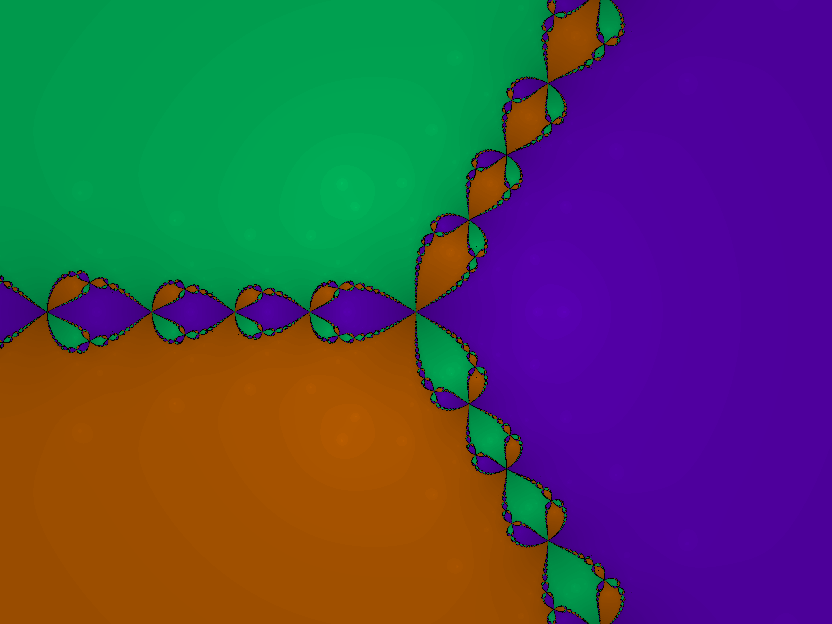
\includegraphics[width=0.95\textwidth]{compdyn01.png}
  \caption{Convergence diagram for $z^3-1$}
\end{figure}

We have many different stable behaviours of this dynamical system, but the boundary is very chaotic. For example, if we consider $p(z) = z^4-2z^2+9$, note that if $z \in \R$, then $f(z) \in \R$. However, the four roots of $p$ are all complex, and so Newton's method will fail to work for $z_0 \in \R$, and this can be seen in the following image:
\begin{figure}[H]
  \centering
  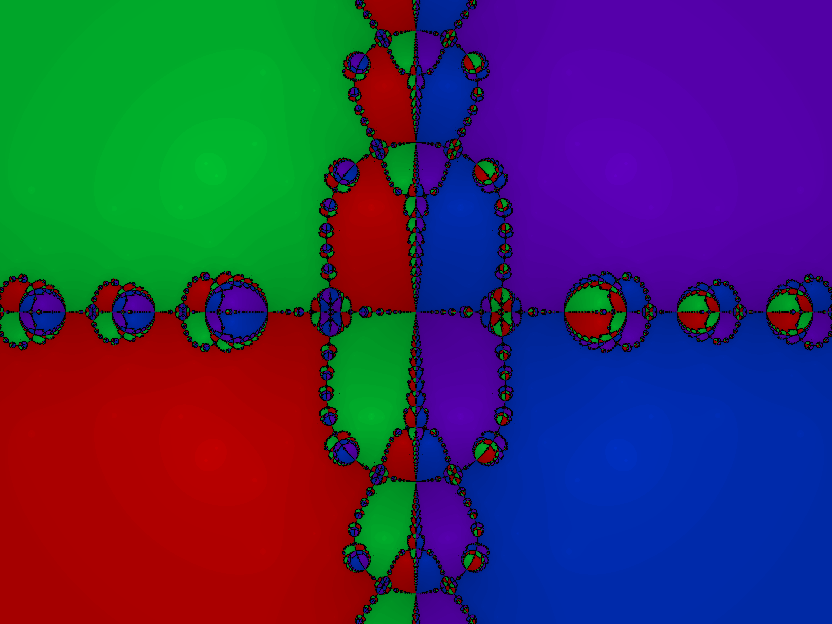
\includegraphics[width=0.95\textwidth]{compdyn02.png}
  \caption{Convergence diagram for $z^4-2z^2+9$}
\end{figure}

\subsection{Applications Motivation: Fixed Point Problems}
Gravitational Lensing: Suppose we have $n$ point masses in a plane perpendicular to the line of sight, and we are observing an object at the origin of this plane, identified with the complex plane. Call the points $z_1, \ldots, z_n$, with masses $\sigma_1, \ldots, \sigma_n$ respectively. Then the images of the object at the origin are the solutions to the \emph{lens equation} $z = \sum_{j=1}^n \frac{\sigma_j}{\bar{z} - \bar{z_j}}$. We see this for instance in the following image, courtesy of \texttt{Nasa}
\begin{figure}[H]
  \centering
  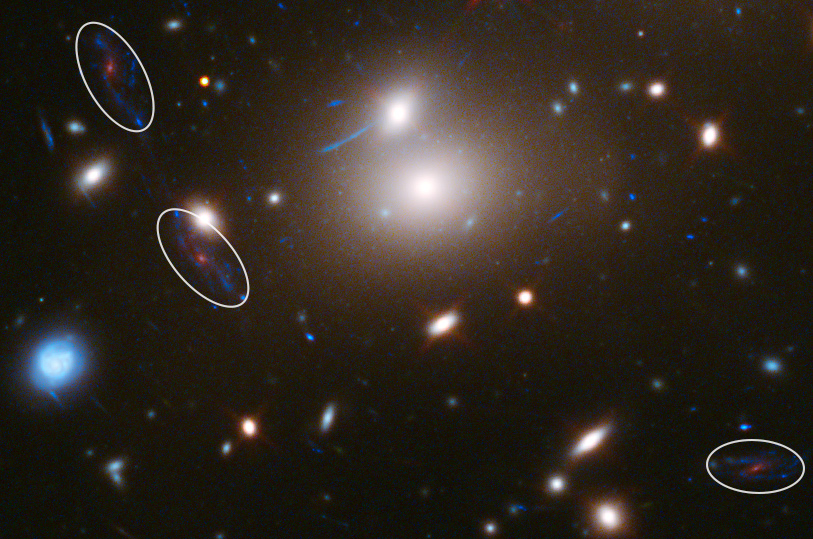
\includegraphics[width=0.95\textwidth]{compdyn03.jpg}
  \caption{The same galaxy appearing 3 times in an image captured by Hubble.}
\end{figure}

For example, if we have a point mass at the origin $n=1, z_1 = 0$. The lens equation gives us images of it at $z = \frac{\sigma_1}{\bar{z}}$, i.e. $|z|^2 = \sigma_1$. The solution is a circle, known as an \emph{Einstein ring}.
\begin{figure}[H]
  \centering
  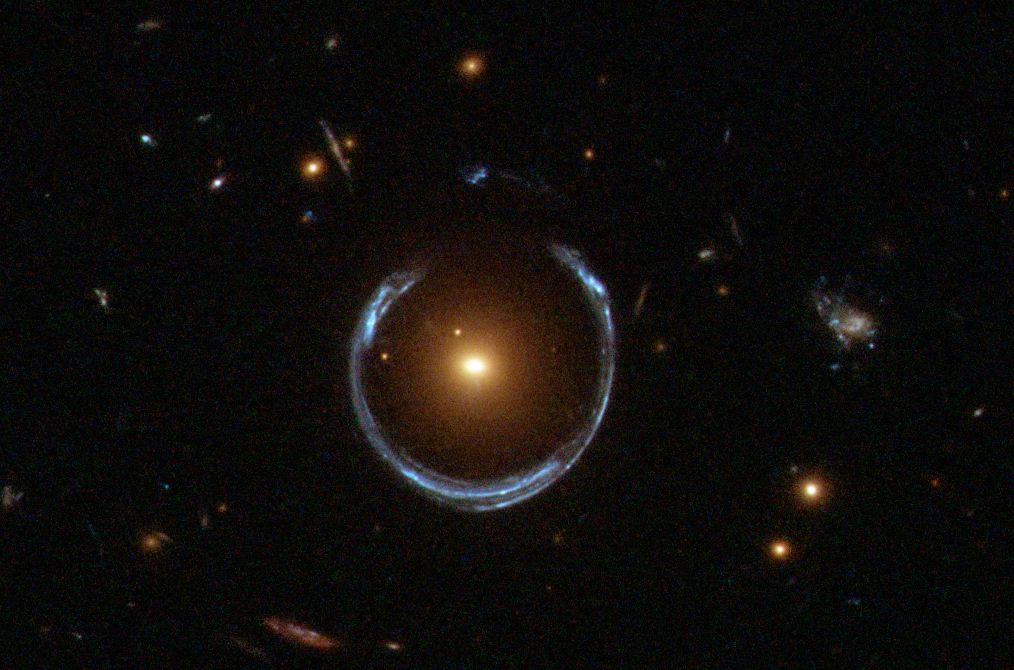
\includegraphics[width=0.95\textwidth]{compdyn04.jpg}
  \caption{An Einstein ring, captured by Hubble.}
\end{figure}

In general, we might want to ask how many images we will see for a give configuration, or perhaps a given number, of point masses.

Define $r(z) \coloneqq \sum_{j=1}^n \frac{\sigma_j}{z-z_j}$, and we are looking for solutions to $z = \overline{r(z)}$, i.e. fixed points of the (non-meromorphic) function $z \mapsto \overline{r(z)}$. These will be among the solutions of the (meromorphic) function $z\mapsto \overline{r(\overline{r(z)})} = r(r(z))$, of degree $n^2$. One can show that it suffices to bound the number of \emph{attracting} fixed points, which will be done in one of the main theorems of this course:

\begin{theorem}
Let $f(z)$ be a rational map of degree $d \geq 2$. Then $f$ has at most $2d-2$ attracting fixed points.
\end{theorem}

There are still open questions related to this application; for example, the following conjecture is still open despite its simplicity:
\begin{conjecture}[(Lee, Lerario, Lundberg)]
If $p$ is a polynomial of degree $n$, $q$ a polynomial of degree $m$, and $n>m$, then the number of solutions to $p(z) = \overline{q(z)}$ is bounded above by $2m(n-1)+n$.
\end{conjecture}

\subsection{Where We're Heading}
Define $f_c(z) \coloneqq z^2+c$, where $c \in \C$. \emph{The Mandelbrot Set} $M \coloneqq \{c \in \C : |f_c^n(0)|\nrightarrow\infty as n\to\infty\}$.
\begin{figure}[H]
  \centering
  
\includegraphics[width=0.95\textwidth]{compdyn05.png}
  \caption{The Mandelbrot set, generated by me.}
\end{figure}

\section{Complex Basics}
\subsection{The Riemann Sphere}
The \emph{Riemann Sphere} $\hat{\C}$ is the one-point compactification of $\C$, given by adding a point at $\infty$. The basis of this topology around $\infty$ are the complements of the closed discs in $\C$.

\begin{definition}
A \emph{domain} in the Riemann sphere is any open connected subset of $\hat{\C}$.
\end{definition}
We can then think about \emph{maps of the Riemann sphere}, which are rational maps of the form $f(z) = \frac{p(z)}{q(z)}$, where $p, q$ are polynomials with no common roots. We define the \emph{degree} of $f$ to be the maximum of $\deg p, \deg q$.

\begin{definition}
We say that $f : \hat{\C} \to \hat{\C}$ is \emph{holomorphic at $\infty$} if $f(1/z)$ is meromorphic on a neighbourhood of 0.
\end{definition}

\begin{lemma}[Identity Principle]
Let $f: D \to D$ be a holomorphic, non-constant map on a domain $D$ in $\hat{\C}$. Then for any $w \in D, f^{-1}(w)$ is discrete. In particular, if $D = \hat{\C}$, then $f^{-1}(w)$ is finite.
\end{lemma}
\begin{proof}
First, composing with a M\"obius map, we may assume $w = 0$. By the principle of isolated zeros, $\forall z \in \hat{\C}$, there is some disc $D_z \ni z$ such that either $f \equiv 0$ on  on $D_z$ or $f$ is nonzero on $D_z \setminus \{z\}$.

Let $V \coloneqq \bigcup_{f = 0 \text{ on } D_z} D_z$, $W \coloneqq \bigcup_{f \neq 0 \text{ on } D_z} D_z$

Then $V \cup W = D$, these sets are open, and $V \cap W = \emptyset$. Since $D$ is connected, $V$ and $W$ cannot disconnect $D$, so one of $V$ and $W$ is empty. $f$ is nonconstant, so $V = \emptyset$, and so the zeros are discrete. As $\hat{\C}$ is compact, any discrete subset is finite.
\end{proof}

\begin{proposition}
Let $f: \hat{\C} \to \hat{\C}$ be a holomorphic, non-constant map. Then $f$ is a non-constant rational function; that is, there exist $a_1, \ldots, a_m, b_1, \ldots b_n \in \C$, and $c \in \C^{\times}$ such that:
\begin{align*}
f(z) = \frac{c(z-a_1)\ldots(z-a_m)}{(z-b_1)\ldots(z-b_n)}
\end{align*}
\end{proposition}

\begin{proof}
Replace by $\frac{1}{f}$ if necessary to assume $f(\infty) \in \C$. By the identity principle, $f^{-1}(\infty)$ is a finite subset of $\C$. Call it $\{b_1, \ldots, b_n\}$. Near each $b_j$, we have a local expansion of $f$ as $f(z) = \sum_{i=-k}^\infty a_{j,i}(z-b_j)^i$. Set $Q_j(z) = \sum_{i=-k}^{-1} a_{j,i}(z-b_j)^i$, each $Q_j$ is a rational function and $g \coloneqq f - (Q_1 + \ldots + Q_n)$ has only removable singularities. So $g(\hat{\C}) \subseteq \C$. Since $\hat{\C}$ is compact, $g(\hat{\C})$ is a compact, proper, open subset of $\C$ $\contr$ (by Heine-Borel). Therefore $g$ is constant, and $f$ is rational.
\end{proof}

\subsection{The Derivative at Infinity}
Caution: there is not a globally well defined notion of a derivative of $f:\hat{\C} \to \hat{\C}$, since we can change coordinates in many different ways. However, if $f(\infty) = \infty$, then we do, as the local derivative is independent of choice of coordinates. In this case, we define $f'(\infty)$ to be the derivative at 0 of $\frac{1}{f(1/z)}$.

\subsection{Uniformizations}
We say a group $\Gamma$ acts \emph{properly discontinuously} on a set if all points $p$ have a neighbourhood $N \ni p$ with $g(N) \cap h(N) = \emptyset$ for all $g \neq h \in \Gamma$

\begin{theorem}[Uniformization in $\hat{C}$]
  Let $U$ be a domain in $\hat{C}$. Then the universal cover $\tilde{U}$ of $U$ is either $\hat{\C}$, $\C$, or $\D$, and $U \simeq \tilde{U}/\Gamma$ for some subgroup $\Gamma \leq \Aut(\tilde{U})$ which acts properly discontinuously.
\end{theorem}

We now consider the different cases:
\begin{itemize}
  \item Universal Cover $\hat{\C}$: $\Aut(\hat{C}) = \{$M\"obius transformations$\}$

  All M\"obius transformations have at least one fixed point. So if $\Gamma$ acts properly discontinuously on $\hat{C}$, $\Gamma$ must be $\{\id\}$, and as such $U = \tilde{U} = \hat{C}$.

  \item Universal Cover $\C$: $\Aut(\C) = \{$M\"obius transformations fixing $\infty\}$

  These transformations are the linear maps, i.e. $f(z) = az+b, a \neq 0$. If a non-identity map lies in $\Gamma$, then it has no fixed point, and hence $az+b=z$ has no solutions, i.e. $a=1, b \neq 0$. So $\Gamma$ consists of the translations, and we can identify $g \in \Gamma$ with $g(0) \in \C$.

  $\Gamma \leq \C$ consists of isolated points, so $\Gamma = \{\id\}, \angle{\omega}$ for some $\omega \in \C$, or a lattice $\Lambda$.

  These correspond respectively to $U \simeq \C, U \simeq \C^\times$, and a complex torus (which is not a subdomain of $\C$).

  \item Universal Cover $\D$: $\Aut(\D) = \left\{e^{\im\theta} \frac{z-\omega}{1-\bar{\omega}z} : \theta \in \R, \omega \in \D\right\}$.

  All the rest! Any domain which omits at least three points of $\hat{\C}$ has the disc as its universal cover. This gives a lot of different subgroups of $\Aut(\D)$ - we won't study which ones are possible in this course.
\end{itemize}

\begin{definition}
  We say a domain $U \subseteq \hat{C}$ is \emph{hyperbolic} if it has universal cover $\D$, or equivalently if it omits at least 3 points.
\end{definition}

If $U$ is a hyperbolic domain, then the covering maps $\tilde{U} \to U$ are holomorphic. So if $f:U \to V$ is a holomorphic map between hyperbolic domains, then its lifted map $g$ is also holomorphic. $g$ is also unique up to a choice of an element of $\Gamma_V$

\begin{theorem}[Picard Theorem]
  If $U$ is a hyperbolic domain, and $f : \C \to U$ is holomorphic, then $f$ is constant.
\end{theorem}
\begin{proof}
  The following diagram commutes:
  \begin{tikzcd}
    \C \arrow{d}{\id} \arrow{r}{g} & \D \arrow{d}{\pi_U} \\ \C \arrow{r}{f} & U
  \end{tikzcd}

  So $g$ is a holomorphic function from $\C$ to $\D$, so bounded, so constant by Liouville's theorem. Hence $f$ must also be constant.
\end{proof}

In fact, there are no non-constant holomorphic maps from $\hat{C}, \C, \C^\ast$ to any hyperbolic domain.

Recall that the hyperbolic (or Poincar\'e) distance between any two points on the disc is the infimum along smooth curves $\gamma : [a,b] \to \D$ which connect the two points of the length value:\[ \ell(\gamma) = \int_a^b \frac{2}{1-|\gamma(t)|^2}|\gamma'(t)| dt\]

Using the origin and automorphisms, one computes that the distance function is given by \[d(x,y) = \frac{\log(1+R)}{\log(1-R)}\] where $R = \left|\frac{y-x}{1-xy}\right|$.

\begin{definition}[Hyperbolic/Poincar\'e metric of a hyperbolic domain]
  Taking the covering map $\pi:\D\to U$ for $U$ a hyperbolic domain to be a local isometry, we define a unique metric on $U$ known as the hyperbolic/Poincar\'e metric on $U$.
\end{definition}

\begin{theorem}[Pick Theorem]
  The $f:U\to V$ be a holomorphic map of hyperbolic domains $U, V \subset \hat{\C}$ with Poincar\'e metrics $\rho_U, \rho_V$ respectively. Then for all $x, y \in U$:\[ \rho_V(f(x), f(y)) \leq \rho_U(x,y)\] with strict inequality unless $f$ lifts to an automorphism of $\D$.
\end{theorem}
\begin{proof}
  By definition of $\rho_U, \rho_V$, it suffices to prove this for $f: \D \to \D$. We want to show that \[\frac{\log(1+R')}{\log(1-R')} \leq \frac{\log(1+R)}{\log(1-R)}\] where
  \begin{align*}
    R &= \left|\frac{y-x}{1-\bar{x}y}\right|,\;\;\;  R' = \left|\frac{f(y)-f(x)}{1-\overline{f(x)}f(y)}\right|
  \end{align*}

  As $\frac{\log(1+x)}{\log(1-x)}$ is strictly increasing, it is sufficient to show $R' \leq R$. Define:
  \begin{align*}
    \sigma_1(z) = \frac{y-z}{1-\bar{y}z},\;\;\;\;\sigma_2(z) = \frac{f(y)-f(z)}{1-\overline{f(y)}f(z)}
  \end{align*}
  Then $\sigma_2 \circ f \circ \sigma_1^{-1} : \D \to \D$ fixes 0. So by Schwarz's lemma, $|\sigma_2 \circ f \circ \sigma_1^{-1}(z)| \leq |z|$, i.e.
  \[
    \left|\frac{f(y)-f(x)}{1-\overline{f(y)}f(x)}\right| \leq \left|\frac{y-x}{1-\bar{y}x}\right|
  \]
by setting $\sigma_1^{-1}(z) = x$. The statement with strict inequality follows similarly.
\end{proof}

Thus all maps of hyperbolic domains are (weakly) contracting with respect to the hyperbolic metric. This is in contrast to the non-hyperbolic case, where we can have things like $f:\C \to \C, z \mapsto 2z$ which is expanding, or $g:\hat{C} \to \hat{C}, z\mapsto z+1$, which has expansion and contraction at the same time in different regions.

\section{What is a reasonable notion of stable/predictable behaviour under iteration?}

For example, take $f(z) = z^2$, so that $f^n(z) = z^{2^n}$. If $|z| > 1$, then $|f^n(z)| = |z|^{2^n} \to \infty$. On the other hand, if we start with a point inside the unit disc, then $|f^n(z)| \to 0$. This is a stable property - if $z$ goes off to $\infty$ or $0$ under iteration of $f$, then $z+\epsilon$ for $|\epsilon|$ small also goes off towards $\infty$ or 0 respectively.

In contrast, if $|z|=1$, then we do not have this stable behaviour.

\begin{definition}
  Let $S, T$ be metric spaces and $f_n : S \to T$ a sequence of continuous maps. We say that $\{f_n\}$ \emph{converges locally uniformly} if for all compact $K \subset S$ and all $\epsilon >0$ there exists $N \in \N$ such that
  \[
    \sup_{z \in K} d_T(f_n(z), f_m(z)) < \epsilon
  \]
  for all $n, m \geq N$.

  We say that $\{f_n\}$ \emph{diverges locally uniformly} if for all compact $K \subset S$ and compact $K' \subset T$, we have $N \in \N$ such that $f_n(K) \cap K' = \emptyset$ for all $n \geq N$.
\end{definition}

\underline{Example:} Let $p(z) = a_dz^d + \ldots + a_0 \in \C[z]$ a polynomial, with sequence of iterates $\{p^n(z) : n \in \N\}$. If $|z| \gg \max\{|a_d|, \ldots, |a_0|\}$, then $|p(z)| \approx |a_dz^d|$. So $|p^n(z)| \to \infty$ as $n \to \infty$. Considering $p:\hat{\C} \to \hat{\C}$, the sequence $\{p^n(z)\}$ converges locally uniformly on a neighbourhood of $\infty$.

Note that the definition of $S, T$ matter - if we consider $p:\C \to \C$ instead then the sequence of iterates $\{p^n(z)\}$ diverges locally uniformly on the complement of some large disc.

\begin{definition}
  A family $\mathcal{F}$ of continuous functions $f: S \to T$ is \emph{normal} if every sequence in $\mathcal{F}$ has a subsequence which is either locally uniformly convergent or locally uniformly divergent.
\end{definition}

\begin{lemma}
  Let $U, V$ be domains and $\mathcal{F}$ a normal family of holomorphic maps $U \to V$. Then any sequence $\{f_n\}$ in $\mathcal{F}$ has a subsequence which converges to a holomorphic limit $g: U \to \bar{V}$, where $\bar{V}$ is the closure of $V$ in the Riemann sphere.
\end{lemma}
\begin{proof}
  $\mathcal{F}$ is normal, so pass to a subsequence of holomorphic maps to assume locally uniform convergence or divergence.

  If $\{f_n\}$ converges locally uniformly, then $\bar{V}$ compact implies we have a limit function $g: U \to \bar{V}$, by taking $K = \{\text{pt}\}$ in the definition. By the Weierstrass uniform convergence theorem, this is holomorphic.

  If $\{f_n\}$ diverges locally uniformly, then for any compact $K \subset U$, we have some convergent subsequence $f_{n_K}(z) \to z_0 \in \partial V$ for any choice of $z \in K$. If $U, V$ are hyperbolic, then by Pick's theorem, all elements of $K$ converge to $z_0$, and so we have local uniform convergence to the constant function at $z_0$. If $U, V$ are not hyperbolic, we may shrink $U$ slightly to still contain $K$, but be hyperbolic $U_0$ with compact closure in $U$.
  By local divergence, we can remove points from $V$ and initial elements of the sequence $\{f_n\}$ to assume $V$ is hyperbolic.
\end{proof}

\underline{Example:} $f(z) = z^2$. $\mathcal{F} \coloneqq \{f^n(z) : n \in \N\}$.

$\hat{\C} \setminus \bar\D$ is a hyperbolic domain, and $f:\hat\C\setminus\bar\D\to\hat\C\setminus\bar\D$, and the iterates $\{f^n(z)|_{\hat\C\setminus\bar\D}\}$ converge locally uniformly to the constant map at $\infty$. Similarly, $\{f^n(z)|_\D\}$ converge locally uniformly to the constant map at 0.

These sets are maximal for these behaviours, i.e. $\{f^n\}$ is a normal family on $\D$ and on $\hat\C\setminus\bar\D$ but on no larger set. If $|z_0| = 1$, then we have for any neighbourhood of $z_0$, some points go to infinity and some go to zero, and so there can be no holomorphic limit of iterates on any neighbourhood of $z_0$.

\section{A More Useful Criterion for Normality}
\textbf{Definition.} A family $\mathcal{F}$ of continuous functions $S \to T$ is \emph{equicontinuous} if, for all $\epsilon > 0$ there is $\delta >0$ such that, for all $f \in \mathcal{F}$ and all $s, t \in S$:
\[d_s(s,t) < \delta \implies d_T(f(s), f(t)) < \epsilon\]

\begin{theorem}[Arzel\`a-Ascoli in $\hat\C$]
  A family $\mathcal{F}: S \to T$ of continuous maps of domains $S, T \subset \hat\C$ has the property that all sequences have a locally uniformly convergent subsequence if and only if the following are both satisfied:
  \begin{itemize}
    \item $\mathcal{F}$ is equicontinuous on any compact subset of $S$, and
    \item For all $z \in S, \{f(z):f \in \mathcal{F}\}$ lies in a compact subset of $T$.
  \end{itemize}
\end{theorem}
\begin{proof}
  The forwards direction is left as an exercise.

  For the reverse direction, since $S, T \subseteq \hat\C$, we can fix a countable dense subset $\{z_k\}$ of $S$. Fix a sequence $\{f_n\}$ of elements of $\mathcal{F}$. We can find a set of indices $\{n_{ij}\}$ such that:
  \begin{align*}
    &n_{11} < n_{12} < n_{13} < \ldots < n_{1j} < \ldots\\
    &n_{21} < n_{22} < n_{23} < \ldots < n_{2j} < \ldots\\
    &\;\;\;\vdots\\
    &n_{i1} < n_{i2} < n_{i3} < \ldots < n_{ij} < \ldots\\
  \end{align*}
  so that each row is contained in the previous as a subsequence, and $\lim\limits_{j \to \infty} f_{n_{kj}}(z_k)$ exists for each $k$.

  The diagonal sequence $g_k \coloneqq f_{n_{kk}}$ is strictly increasing in index, and for each $k$, eventually contained in the $k\th$ row. So $g_k$ converges at each $z_k$.

  Consider now $K$, a compact subset of $S$. Given $\epsilon > 0$ there is $\delta >0$ such that, for all $x,y \in K$ and all $g_k$, $d_S(x, y) < \delta \implies d_T(g_k(x), g_k(y)) < \epsilon/3$.

  Cover $K$ by finitely many $\delta/2$ diameter neighbourhoods, selecting some $z_k$ for each of these neighbourhoods.

  Given $z \in K$, we have some $z_k$ with $\delta$, and there are only finitely many $z_k$ in this set, so in fact we can find $N$ such that $n, m > N$ implies $d_T(g_n(z_k), g_m(z_k)) < \frac{\epsilon}{3}$.

  So we have:
  \begin{align*}
    d_T(g_n(z), g_m(z)) &\leq d_T(g_n(z), g_m(z_k)) + d_T(g_n(z_k), g_m(z_k)) + d_T(g_m(z_k), g_m(z))\\
    &< \epsilon/3 + \epsilon/3 + \epsilon/3\\
    &= \epsilon
  \end{align*}
  Since this holds for all $z \in K$, we have locally uniform convergence as claimed.
\end{proof}
\addtocounter{theorem}{-1}
\begin{corollary}
  If $T$ is compact, a family of continuous maps from $S$ to $T$ is normal if and only if it is equicontinuous on compact subsets.
\end{corollary}

This brings us to the critical takeaway applicable to dynamics:
\begin{theorem}[Montel's theorem]
  Let $U, V$ be domains with $V$ hyperbolic. Then the family of holomorphic maps from $U$ to $V$ forms a normal family.
\end{theorem}
\begin{proof}
  Suppose first that $U$ is hyperbolic. By Pick's theorem, the family is equicontinuous.

  If $\exists x \in U$ such that $\{f(x) : f \in \mathcal{F}\}$ is in some compact $K \subseteq V$, then again by Pick's theorem, the same is true for all points in $U$. So by Arzel\`a-Ascoli, we have a normal family.

  Otherwise, we can fix $x \in U, y \in V$, and an infinite sequence $\{f_n\}\subseteq \mathcal{F}$ such that $\rho_V(f_n(x), y) \to \infty$ as $n \to \infty$. Fix compact $K \subseteq U, K'\subseteq V$, noting that $\rho_U(x, K), \rho_V(y, K')$ are finite, we have by Pick's theorem that $f_n(K) \cap K' = \emptyset$ for all $n$ sufficiently large. So this sequence diverges locally uniformly, and again we have a normal family.

  In the case where $U$ is not hyperbolic, then $\mathcal{F}$ consists of constant maps.

  If there is a subsequence with images in a compact set, then we have a locally uniformly convergent subsequence.

  If not, then only finitely many of these maps have image in any compact set - we have locally uniform divergence.
\end{proof}

\underline{Example:} $f(z) = z^2$. We've seen that $\{f^n(z) : n \in \N\}$ form a normal family on $\D$ and $\hat\C\setminus\bar\D$, by manual computation. But since $f^n(\D) \subseteq \D, f^n(\hat\C\setminus\bar\D)\subseteq\hat\C\setminus\bar\D$, the iterates of $f$ must form a normal family on these domains because the image spaces are hyperbolic.

More generally, if $U \subseteq \hat\C$ is a hyperbolic domain, either $\{f^n(U) : n \in \N\}$ covers all but at most 2 points of $\hat\C$, or the iterates of $f$ form a normal family on $U$.

\section{Degree and Ramification}
\begin{definition}
  A continuous map $f:U \to V$ of topological spaces is \emph{proper} if for all $K \subset V$, $f^{-1}(K)$ is compact in $U$.
\end{definition}
\addtocounter{theorem}{-1}
\begin{lemma}
  Let $f:U\to V$ be continuous. If $U$ is compact and $V$ is Hausdorff, then $f$ is proper.
\end{lemma}
\begin{proof}
  Let $K \subseteq V$ be compact. $V$ is Hausdorff $\implies$ $K$ is closed, so $V \setminus K$ is open $\implies f^{-1}(V\setminus K)$ is open (as $f$ is continuous). So $f^{-1}(K) = U \setminus f^{-1}(V\setminus K)$ is closed, and so compact as it is a closed subset of a compact set. So $f$ is proper.
\end{proof}

Recall from complex analysis the concept of local degree/ramification: if $f$ is holomorphic on a neighbourhood of $z_0$, with $f(z_0) = w_0$, then locally we have an expansion\[f(z) = w_0 + (z-z_0)^eg(z-z_0)\] where $g(z-z_0)$ is nonzero at $z_0$, and holomorphic on a neighbourhood of $z_0$. Then $e$ is the local degree/ramification index at $z_0$. If $e > 1$, then $z_0$ is said to be critical.

Let $U, V$ be domains in $\hat\C$.
\addtocounter{theorem}{-1}
\begin{proposition}
  If $f:U \to V$ is a proper holomorphic map, then $f$ has a well defined degree on $U$, equal to\[\sum_{z \in U: f(z) = w} e_z\] for any $w \in V$, where $e_z$ is the ramification index of $f$ at $z$.
\end{proposition}
Note that this is independent of $w$, and by Lemma \textbf{5.1}, all rational maps have well-defined degree!
\addtocounter{theorem}{-1}
\begin{theorem}[Riemann-Hurwitz]
  Let $f:U \to V$ be proper of degree $d$. Then\[\chi(U) = d\chi(V) - \sum_{p\in V}(e_p-1)\] where $e_p$ is the ramification index of $f$ at $p$ and $\chi$ is the Euler characteristic.
\end{theorem}
We will take both of these theorems for granted - they follow immediately from the corresponding statements for compact sets.

\begin{corollary}
  Any degree $d$ rational function $f$ has $2d-2$ critical points, counting multiplicity.
\end{corollary}
\begin{proof}
  $\chi(\hat\C) = 2$, and use Riemann-Hurwitz.
\end{proof}
\begin{corollary}
  If $U, V$ have $\chi(U) = \chi(V) = 0$, (e.g. annuli, punctured discs), then any proper holomorphic $f:U \to V$ is unramified.
\end{corollary}
\end{document}
